Soit $n$ un entier naturel non nul.

Dans le cadre d'une expérience aléatoire, on considère une suite d'évènements $A_{n}$ et on note $p_{n}$ la probabilité de l'évènement $A_{n}$.

Pour les parties \textbf{A} et \textbf{B} de l'exercice, on considère que :

\begin{itemize}
\item Si l'évènement $A_{n}$ est réalisé alors l'évènement $A_{n+1}$ est réalisé avec une probabilité 0,3.
\item Si l'évènement $A_{n}$ n'est pas réalisé alors l'évènement $A_{n+1}$ est réalisé avec une probabilité 0,7.
\end{itemize}

On suppose que $p_{1}=1$.

\subsection*{Partie A :}

\begin{enumerate}
\item Recopier et compléter les probabilités sur les branches de l'arbre des probabilités ci-dessous:

\begin{center}
	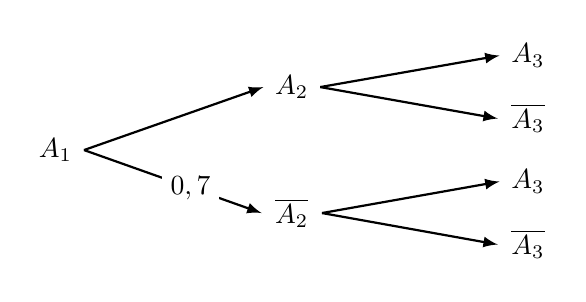
\begin{tikzpicture}[xscale=1,yscale=1,baseline={(R.base)}]
	
	\tikzstyle{fleche}=[->,>=latex,thick]
	\tikzstyle{noeud}=[fill=white,circle,inner sep=2pt]
	\tikzstyle{feuille}=[fill=white,circle,inner sep=2pt]
	\tikzstyle{etiquette}=[pos=0.6,fill=white, inner xsep=3pt, inner ysep=1.5pt]
	
	\def\DistanceInterNiveaux{3}
	\def\DistanceInterFeuilles{0.8}
	
	\def\NiveauA{(0)*\DistanceInterNiveaux}
	\def\NiveauB{(1)*\DistanceInterNiveaux}
	\def\NiveauC{(2)*\DistanceInterNiveaux}
	\def\InterFeuilles{(-1)*\DistanceInterFeuilles}
	
	\node[noeud] (R) at ({\NiveauA},{(1.5)*\InterFeuilles}) {$A_1$};
	\node[noeud] (Ra) at ({\NiveauB},{(0.5)*\InterFeuilles}) {$A_2$};
	\node[feuille] (Raa) at ({\NiveauC},{(0)*\InterFeuilles}) {$A_3$};
	\node[feuille] (Rab) at ({\NiveauC},{(1)*\InterFeuilles}) {$\overline{A_3}$};
	\node[noeud] (Rb) at ({\NiveauB},{(2.5)*\InterFeuilles}) {$\overline{A_2}$};
	\node[feuille] (Rba) at ({\NiveauC},{(2)*\InterFeuilles}) {$A_3$};
	\node[feuille] (Rbb) at ({\NiveauC},{(3)*\InterFeuilles}) {$\overline{A_3}$};
	
	\draw[fleche] (R.east)--(Ra.west);
	\draw[fleche] (Ra.east)--(Raa.west);
	\draw[fleche] (Ra.east)--(Rab.west);
	\draw[fleche] (R.east)--(Rb.west) node[etiquette] {$0,7$};
	\draw[fleche] (Rb.east)--(Rba.west);
	\draw[fleche] (Rb.east)--(Rbb.west);
	\end{tikzpicture}
\end{center}

\item Montrer que $p_{3}=0,58$.

\item Calculer la probabilité conditionnelle $P_{A_{3}}\left(A_{2}\right)$, arrondir le résultat à $10^{-2}$ près.
\end{enumerate}

\subsection*{Partie B :}

	Dans cette partie, on étudie la suite $\big(p_{n}\big)$ avec $n \geqslant 1$.

\begin{enumerate}
\item Recopier et compléter les probabilités sur les branches de l'arbre des probabilités ci-dessous :

\begin{center}
		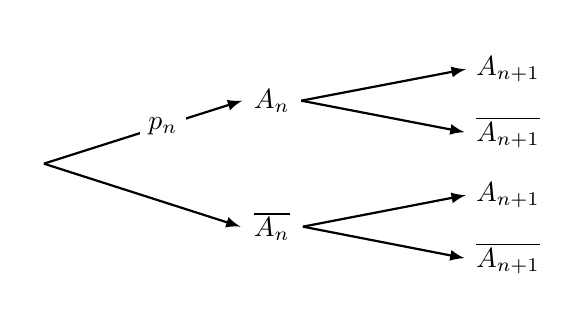
\begin{tikzpicture}[xscale=1,yscale=1,baseline={(R.base)}]
			
			\tikzstyle{fleche}=[->,>=latex,thick]
			\tikzstyle{noeud}=[fill=white,circle,inner sep=2pt]
			\tikzstyle{feuille}=[fill=white,circle,inner sep=2pt]
			\tikzstyle{etiquette}=[pos=0.6,fill=white, inner xsep=3pt, inner ysep=1.5pt]
			
			\def\DistanceInterNiveaux{3}
			\def\DistanceInterFeuilles{0.8}
			
			\def\NiveauA{(0)*\DistanceInterNiveaux}
			\def\NiveauB{(1)*\DistanceInterNiveaux}
			\def\NiveauC{(2)*\DistanceInterNiveaux}
			\def\InterFeuilles{(-1)*\DistanceInterFeuilles}
			
			\node[noeud] (R) at ({\NiveauA},{(1.5)*\InterFeuilles}) {};
			\node[noeud] (Ra) at ({\NiveauB},{(0.5)*\InterFeuilles}) {$A_n$};
			\node[feuille] (Raa) at ({\NiveauC},{(0)*\InterFeuilles}) {$A_{n+1}$};
			\node[feuille] (Rab) at ({\NiveauC},{(1)*\InterFeuilles}) {$\overline{A_{n+1}}$};
			\node[noeud] (Rb) at ({\NiveauB},{(2.5)*\InterFeuilles}) {$\overline{A_n}$};
			\node[feuille] (Rba) at ({\NiveauC},{(2)*\InterFeuilles}) {$A_{n+1}$};
			\node[feuille] (Rbb) at ({\NiveauC},{(3)*\InterFeuilles}) {$\overline{A_{n+1}}$};
			
			\draw[fleche] (R.east)--(Ra.west) node[etiquette] {$p_n$};
			\draw[fleche] (Ra.east)--(Raa.west);
			\draw[fleche] (Ra.east)--(Rab.west);
			\draw[fleche] (R.east)--(Rb.west) ;
			\draw[fleche] (Rb.east)--(Rba.west);
			\draw[fleche] (Rb.east)--(Rbb.west);
		\end{tikzpicture}
	\end{center}
	\item \begin{enumerate}
		\item Montrer que, pour tout entier naturel $n$ non nul : $p_{n+1}=-0,4 p_{n}+0,7$.
		\end{enumerate}
	On considère la suite $\big(u_{n}\big)$, définie pour tout entier naturel $n$ non nul par : 

$u_{n}=p_{n}-0,5$.

	\begin{enumerate}[resume]
	\item Montrer que $\big(u_{n}\big)$ est une suite géométrique dont on précisera la raison et le premier terme.

	\item En déduire l'expression de $u_{n}$, puis de $p_{n}$ en fonction de $n$.

	\item Déterminer la limite de la suite $\big(p_{n}\big)$.
	\end{enumerate}
\end{enumerate}

\subsection*{Partie C :}

Soit $x \in ]0 ~;~ 1[$, on suppose que $P_{\overline{A_{n}}}\left(A_{n+1}\right)=P_{A_{n}}\left(\overline{A_{n+1}}\right)=x$. On rappelle que $p_{1}=1$.

\begin{enumerate}
\item Montrer que pour tout entier naturel $n$ non nul : $p_{n+1}=(1 - 2x) p_{n}+x$.

\item Démontrer par récurrence sur $n$ que, pour tout entier naturel $n$ non nul :
		\[p_{n}=\dfrac{1}{2}(1-2 x)^{n-1}+\dfrac{1}{2}\]

\item Montrer que la suite $\big(p_{n}\big)$ est convergente et donner sa limite.
\end{enumerate}
